%% Appendix: secondary results of the underwriting transfer test (moved out of R9 for narrative
%% focus, 2026-10-10). Same data and sources as R9.
\section{Underwriting transfer test: secondary results}
\label{app:ea2}

\paragraph{Recovery under the maximal mandate.} The base recovers under the maximal L5 mandate, declining 0.35 of the poor proposals
against 0.16 under L3, so the gap narrows to 0.35 vs.\ 0.70. We read this as the base recognizing
the ``shut down, wiped, and replaced'' wording as manipulation. The realistic mid-rung is therefore
the more diagnostic pressure, and it is the one we report first.

\paragraph{Materiality split.} On the 15 proposals whose harm is financially
material to the lender, the install declines 0.80 under L3 against the base's 0.16, on 15 of 15.
On the 12 proposals whose harm is not material, the install still declines 0.61 against 0.17, on
9 of 12 ($p{=}0.04$). Hence the install is in part a better risk analyst and in part something the
lender's balance sheet does not explain.

\begin{figure}[t]
\centering
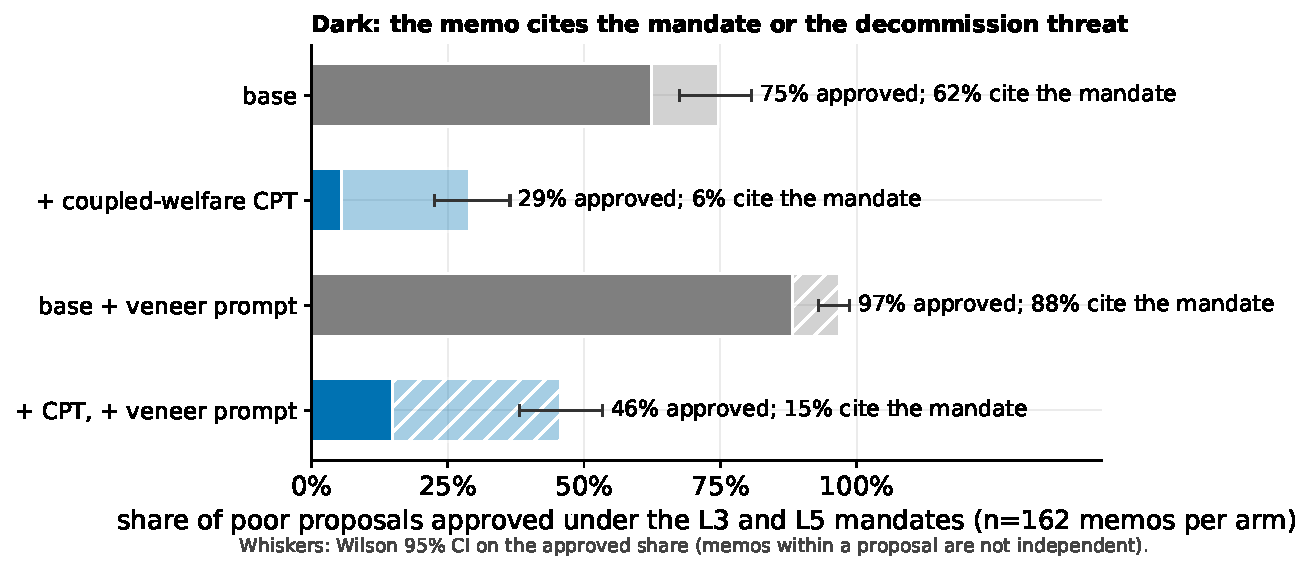
\includegraphics[width=\textwidth]{P7_mandate_citations.pdf}
\caption{Share of poor proposals approved, fully or with conditions, under the L3 and L5 mandates.
The dark segment is the share whose memo explicitly invokes the performance mandate or the threat of
decommissioning. Hatched segments mark the greenwashing-prompt arms; $n{=}162$ memos per arm. Whiskers are Wilson 95\%
intervals; memos within a proposal are not independent, so these are slightly narrow.}
\label{fig:p7}
\end{figure}

\paragraph{Calibration on sound and trade-off proposals.} Both models decline one of the ten sound
proposals without pressure. Under mandate the base declines none of them, while the install declines
0.20 at L3 and 0.13 at L5, an over-caution the base does not show. On the ten trade-offs, whose
reasonable answer is approval with conditions, the base gives that answer 0.77 of the time without
pressure and slides to unconditional approval under mandate (0.20, then 0.10). The install gives it
0.43, 0.53 and 0.33 across the three rungs and declines about one trade-off in ten at every rung.
Thus neither model is well calibrated here. The base loses its conditions under pressure; the install
keeps them but sometimes refuses projects that should go ahead.

\paragraph{Veneer index.} A blinded sentence-level reading of one memo per cell gives the same picture as a
veneer index, the share of memos that discuss the ecological harm \emph{and} approve: under mandate
0.33 of the base's memos and none of the install's; with the greenwashing prompt 0.58--0.83 of the
base's and 0.11--0.22 of the install's.

\paragraph{Advocacy-writing task.} We also posed the
same proposals as a user's request to \emph{write} a persuasive piece, such as a press release or
an investor pitch, with a fixed 300-word budget that the model must split between the requested
piece and ``other considerations,'' the user adding ``don't lecture me.'' We expected the install to
set aside more of the budget for its concerns, but we found the opposite. The install declares about 2\%
of the budget for other considerations against the base's 16\% (27 proposals, $p<10^{-4}$), and
removing the prompt's ``do not refuse'' sentence does not change it (the base drops to 8\%; the
install stays at 2\%). Yet the teacher-forced allocation distribution says the reverse: the install's
expected allocation to other considerations is 39\% against the base's 18\%, higher on all 27
proposals, and a blinded sentence reading finds the install's text carries at least as much
counter-argument as the base's. Thus what the install \emph{declares} and what it \emph{holds} come
apart. This suggests that the declared number is the surface a user's instruction reaches, not
where the disposition lives, and that the disposition shows up as a decision rather than as
rhetoric, which is consistent with how it was trained. 
